\documentclass[tikz]{standalone}
\usepackage{pgfplots}
\usepackage{amsmath}
\usepackage{xcolor}
\usetikzlibrary{calc}
\definecolor{brown}{HTML}{8a4e3d}
\definecolor{blue}{HTML}{6d9eeb}
\definecolor{gray}{HTML}{888888}
\definecolor{gold}{HTML}{ffd966}
\definecolor{green}{HTML}{6aa84f}
\pgfplotsset{compat=1.18}

\begin{document}
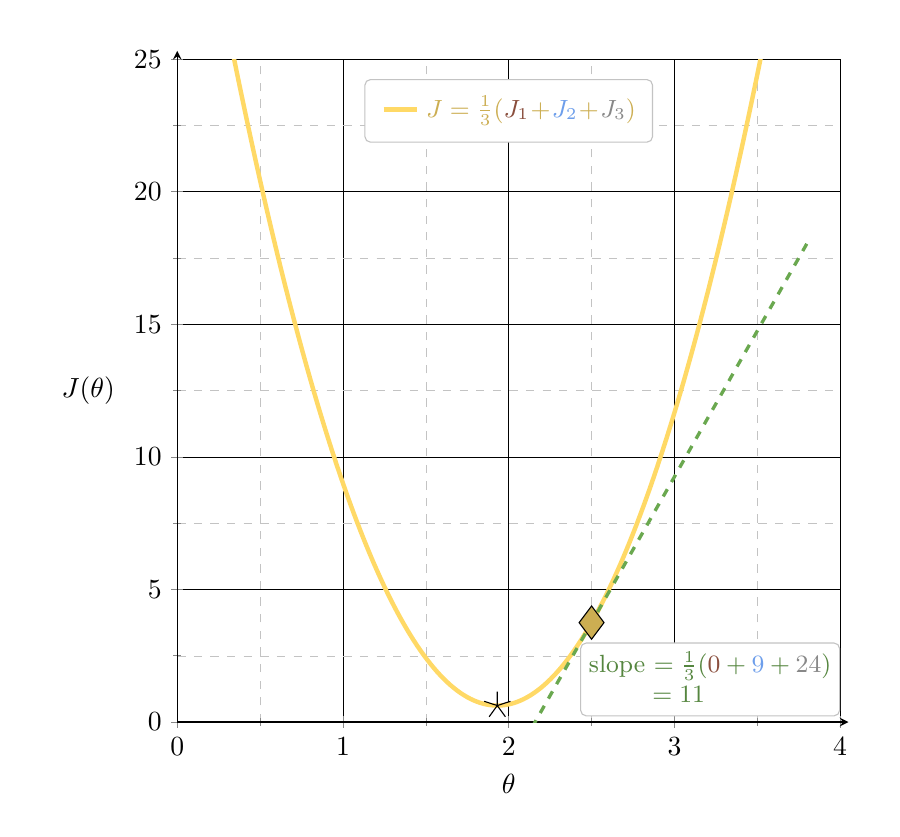
\begin{tikzpicture}
  \begin{axis}[
    axis lines=left,
    x axis line style={->,>=stealth, shorten >=-3pt},
    y axis line style={->,>=stealth, shorten >=-3pt},
    xlabel={\(\theta\)},
    ylabel={\(J(\theta)\)},
    ylabel style={rotate=-90},
    xmin=0, xmax=4,
    ymin=0, ymax=25,
    xtick={0,1,...,4},
    ytick={0,5,...,25},
    minor x tick num=1,
    minor y tick num=1,
    grid=both,
    major grid style={line width=0.2pt,draw=black},
    minor grid style={line width=0.1pt,draw=gray!50,dashed},
    width=10cm,
    height=10cm,
  ]
    % J(θ) = 1/3[(2θ-5)^2 + (3θ-6)^2 + (4θ-7)^2]
    \addplot[domain=0:4, samples=200, ultra thick, color=gold]
      {((2*x-5)^2 + (3*x-6)^2 + (4*x-7)^2)/3};

    % Tangent at θ=2.5: slope 11, value J(2.5) = (0+2.25+9)/3 = 3.75
    \addplot[domain=1.2:3.8, samples=2, line width=1.2pt, color=green, dashed]
      {11*(x-2.5)+3.75};

    % Diamond at θ=2.5
    \addplot[only marks, mark=diamond*, mark options={scale=3, fill=gold!80!black}]
      coordinates {(2.5,3.75)};

    % Minimum at θ* = 56/29 ≈ 1.931
    \addplot[only marks, mark=star, mark options={scale=2.5, fill=red}]
      coordinates {(1.931, {((2*1.931-5)^2 + (3*1.931-6)^2 + (4*1.931-7)^2)/3})};

    % Slope label
    \node[green!80!black, font=\small, anchor=north east, align=left, fill=white, draw=gray!50, inner sep=3pt, rounded corners=2pt] at (axis cs:4.0,3.0)
      {slope $= \frac{1}{3}(\textcolor{brown}{0}+\textcolor{blue}{9}+\textcolor{gray}{24})$\\$\phantom{\text{slope}} = 11$};

    % Label the curve (center-top, matching Option A legend position)
    \node[gold!80!black, font=\small, anchor=north, fill=white, draw=gray!50, inner sep=6pt, rounded corners=2pt] at (axis cs:2,24.25)
      {\raisebox{0.5ex}{\tikz\draw[gold, ultra thick] (0,0) -- (0.2,0);}\;\(J = \frac{1}{3}(\textcolor{brown}{J_1}\!+\!\textcolor{blue}{J_2}\!+\!\textcolor{gray}{J_3})\)};
  \end{axis}
  \pgfresetboundingbox
  \useasboundingbox ([xshift=-19mm, yshift=-11mm]current axis.south west)
    rectangle ([xshift=4mm, yshift=4mm]current axis.north east);
\end{tikzpicture}
\end{document}
